% mnras_template.tex 
%
% LaTeX template for creating an MNRAS paper
%
% v3.0 released 14 May 2015
% (version numbers match those of mnras.cls)
%
% Copyright (C) Royal Astronomical Society 2015
% Authors:
% Keith T. Smith (Royal Astronomical Society)

% Change log
%
% v3.0 May 2015
%    Renamed to match the new package name
%    Version number matches mnras.cls
%    A few minor tweaks to wording
% v1.0 September 2013
%    Beta testing only - never publicly released
%    First version: a simple (ish) template for creating an MNRAS paper

%%%%%%%%%%%%%%%%%%%%%%%%%%%%%%%%%%%%%%%%%%%%%%%%%%
% Basic setup. Most papers should leave these options alone.
\documentclass[fleqn,usenatbib]{mnras}

% MNRAS is set in Times font. If you don't have this installed (most LaTeX
% installations will be fine) or prefer the old Computer Modern fonts, comment
% out the following line
\usepackage{newtxtext,newtxmath}
% Depending on your LaTeX fonts installation, you might get better results with one of these:
%\usepackage{mathptmx}
%\usepackage{txfonts}

% Use vector fonts, so it zooms properly in on-screen viewing software
% Don't change these lines unless you know what you are doing
\usepackage[T1]{fontenc}
\usepackage{ae,aecompl}


%%%%% AUTHORS - PLACE YOUR OWN PACKAGES HERE %%%%%

% Only include extra packages if you really need them. Common packages are:
\usepackage{graphicx}	% Including figure files
\usepackage{amsmath}	% Advanced maths commands
\usepackage{amssymb}	% Extra maths symbols

%%%%%%%%%%%%%%%%%%%%%%%%%%%%%%%%%%%%%%%%%%%%%%%%%%

%%%%% AUTHORS - PLACE YOUR OWN COMMANDS HERE %%%%%

% Please keep new commands to a minimum, and use \newcommand not \def to avoid
% overwriting existing commands. Example:
%\newcommand{\pcm}{\,cm$^{-2}$}	% per cm-squared
\newcommand{\red}[1]{{\textcolor{red}{#1}}}
\newcommand{\green}[1]{{\textcolor{green}{#1}}}
\newcommand{\blue}[1]{{\textcolor{blue}{#1}}}

%%%%%%%%%%%%%%%%%%%%%%%%%%%%%%%%%%%%%%%%%%%%%%%%%%

%%%%%%%%%%%%%%%%%%% TITLE PAGE %%%%%%%%%%%%%%%%%%%

% Title of the paper, and the short title which is used in the headers.
% Keep the title short and informative.
\title[Origin of kinematic misalignment]{SDSS-IV MaNGA: Kinematic misalignment in about 6000 galaxies: revealing the evolutionary pathways leading to offsets between stellar and gas rotation}

% The list of authors, and the short list which is used in the headers.
% If you need two or more lines of authors, add an extra line using \newauthor
\author[C. Duckworth et al.]{Christopher Duckworth,$^{1}$\thanks{E-mail: cd201@st-andrews.ac.uk}
Rita Tojeiro,$^{1}$
Third Author$^{2,3}$
and Fourth Author$^{3}$
\\
% List of institutions
{}$^{1}$School of Physics and Astronomy, University of St Andrews, North Haugh, St Andrews, KY16 9SS, UK\\
$^{2}$Department, Institution, Street Address, City Postal Code, Country\\
$^{3}$Another Department, Different Institution, Street Address, City Postal Code, Country
}

% These dates will be filled out by the publisher
\date{Accepted XXX. Received YYY; in original form ZZZ}

% Enter the current year, for the copyright statements etc.
\pubyear{2019}

% Don't change these lines
\begin{document}
\label{firstpage}
\pagerange{\pageref{firstpage}--\pageref{lastpage}}
\maketitle

% Abstract of the paper
\begin{abstract}
This is a simple template for authors to write new MNRAS papers.
The abstract should briefly describe the aims, methods, and main results of the paper.
It should be a single paragraph not more than 250 words (200 words for Letters).
No references should appear in the abstract.
\end{abstract}

% Select between one and six entries from the list of approved keywords.
% Don't make up new ones.
\begin{keywords}
keyword1 -- keyword2 -- keyword3
\end{keywords}
\section{Introduction}

\section{Data}
\subsection{The MaNGA survey}
Set to complete in 2020, the MaNGA survey is designed to investigate the internal structure of $\sim$10000 galaxies in the nearby Universe. By design, the complete sample is unbiased towards morphology, inclination and colour and provides a near flat distribution in stellar mass. 

MaNGA is one of three programs in the fourth generation of the Sloan Digital Sky Survey (SDSS-IV) which enables detailed kinematics through integral field unit (IFU) spectroscopy. MaNGA uses the SDSS 2.5 meter telescope in spectroscopic mode \citep{gunn2006} with the two dual-channel BOSS spectrographs \citep{smee2013} and the MaNGA IFUs \citep{drory2015}. MaNGA provides spatial resolution on kpc scales (2'' diameter fibres) while covering 3600-10300$\mathring{A}$ in wavelength with a resolving power that varies from R$\sim$1400 at 4000$\mathring{A}$ to R$\sim$2600 at 9000$\mathring{A}$. 

MaNGA observations are covered plate by plate, employing a dithered pattern for each galaxy corresponding to one of the 17 fibre-bundles of 5 distinct sizes. Any incomplete data release of MaNGA should therefore be unbiased with respect to IFU sizes and hence a reasonable representation of the final sample scheduled to be complete in 2020.

The majority of observations contribute to one of the three main subsets: the Primary sample, the Secondary sample and the Colour-Enhanced supplement. All sub-samples observe galaxies to a minimum of $\sim 1.5$ effective radii ($R_{e}$) with the Secondary sample increasing this minimum to $\sim 2.5 R_{e}$. The Colour-Enhanced supplement fills in gaps of the colour-magnitude diagram leading to an approximately flat distribution of stellar mass. A full description of the MaNGA observing strategy is given in \citet{law2015obs,yan2016obs}. 
The raw observations are processed by the MaNGA Data 
Reduction Pipeline (DRP) as described in \citet{law2016drp, yan2016spec}. The fibre flux and inverse variance is extracted from each exposure, which are then wavelength calibrated, flat-fielded and sky subtracted. In this work, we use 6044 galaxies from the eighth MaNGA Product Launch (MPL-8) that are selected in the Primary, Secondary and Colour-Enhanced samples and have non-critical observations. Figure \ref{fig:samp_cons} shows the distribution of stellar mass and redshift of the eighth MaNGA Product Launch (MPL-8) with comparison to the NASA-Sloan Atlas (NSA) catalogue from which MaNGA is targeted and our $\Delta$PA defined sub-sample outlined in \S\ref{sec:samp_sec}.

\begin{figure}
	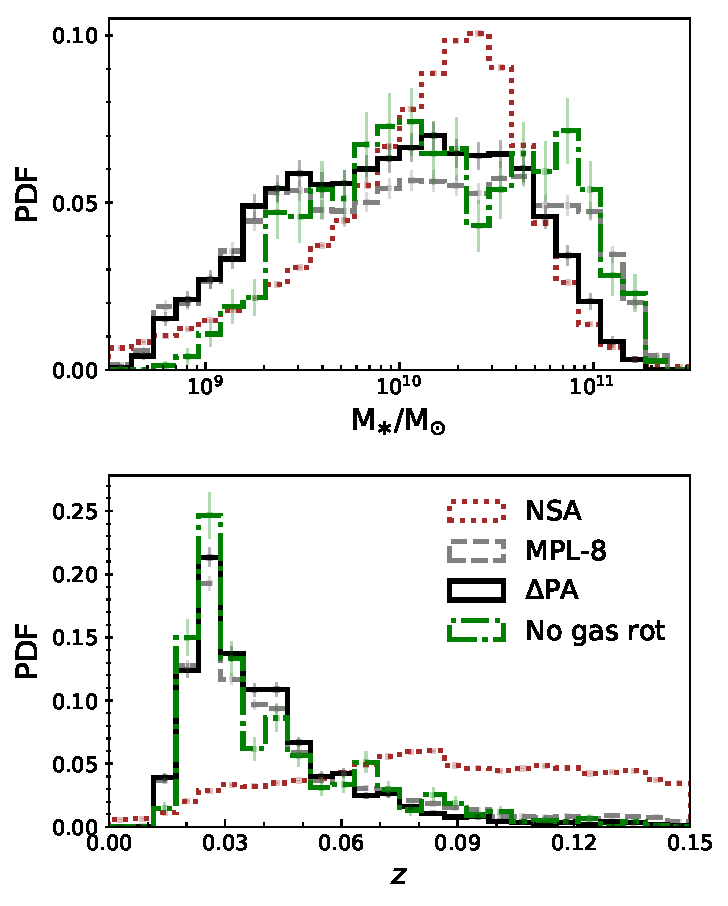
\includegraphics[width=\linewidth]{total_pop/mpl8_pa_nsa_stelmass_z.pdf}
    \caption{Relative frequency distributions of stellar mass and redshift for the NSA target catalogue (brown dotted line), MaNGA MPL-8 (gray dashed line), our $\Delta$PA sub-sample (black solid line) and those with a defined stellar PA but no clear H$\alpha$ rotation (green dot-dashed line). The figure is cut at $z=0.15$ representing the extent of MaNGA targets. Each histogram is given with Poisson errors on each bin.}
    \label{fig:samp_cons}
\end{figure}

\subsection{Spectral fitting for kinematics}
All stellar and H$\alpha$ velocity fields are taken directly from the MaNGA Data Analysis Pipeline \citep[DAP;][for an overview and emission line modelling respectively]{westfall2019, belfoire2019}, we direct the reader to these references, however we summarise the key points here.

The DAP extracts stellar kinematics using the Penalised Pixel-Fitting (pPXF) method \citep{cappellari2004,cappellari2017}. The DAP fits the stellar continuum of each spaxel to extract the line of sight velocity dispersion and then fits the absorption-line spectra from a set of 49 clusters of stellar spectra from the MILES stellar library \citep{sanchez2006,falcon2011}. Before extraction of the mean stellar velocity, the spectra are spatially Voronoi binned to $g$-band \textit{S/N} $\sim$ 10, excluding any individual spectrum with a $g$-band \textit{S/N} < 1 \citep{cappellari2003}. This approach is geared towards stellar kinematics as the spatial binning is applied to the continuum \textit{S/N}, however, we note that unbinned and Voronoi binned velocity maps produce similar results. 

Ionized gas kinematics are extracted by the DAP through fitting a Gaussian to the H$\alpha$-6564 emission line, relative to the input redshift for the galaxy. This velocity is representative for all ionized gas, since the parameters for each Gaussian fit to each emission line are tied during the fitting process. These velocities are also binned spatially by the Voronoi bins of the stellar continuum. 

\subsection{Defining global position angles}
For a complete description of PA fitting and typical error estimation for MaNGA, we direct the reader to Duckworth+19. Here we use a similar process, summarising the key points and highlighting differences with respect to Duckworth+19.

Global position angles (PA) are estimated for both the stellar and ionized gas velocity fields using the \texttt{fit\_kinematic\_pa} routine \citep[see Appendix C of][for a description of the process]{krajnovic2006}. \texttt{fit\_kinematic\_pa} returns the angle (counter-clockwise) of the bisecting line which has greatest velocity change along it. The best fit angle is found by sampling 181 equally spaced steps, so that the output PA will have precision of 0.5$^{\circ}$. By default, \texttt{fit\_kinematic\_pa} returns a PA defined between 0$^{\circ}$ and 180$^{\circ}$, which is indiscriminate towards direction of the blueshifted and redshifted sides. To adjust this, we identify the redshifted side and return PAs defined by the angle to the redshifted side clockwise from the north axis (0-360$^{\circ}$). 

The accuracy of PA fitting is biased by neighbouring galaxies, spectral pixels (spaxels) with spuriously high velocities and inclination. 

Foreground stars are removed during the spectral fitting, however foreground/background galaxies can remain within the IFU footprint. This can be a significant problem for global PA fitting since \texttt{fit\_kinematic\_pa} symmetrizes the velocity fields and interpolates to estimate the PA. Background/small objects can then bias the PA fit for the main target, especially in the instance where they are moving significantly different to the target galaxy. To counteract this, we remove all disconnected regions smaller than $10\%$ of the target galaxy's footprint. 

Spaxels with spuriously high velocities (e.g. > 1000km/s relative to target's central redshift) can also bias PA fits during symmetrization. These often correspond to background galaxies that are connected (on the sky) to the target galaxy's footprint, and hence, we sigma clip the velocity field and remove all spaxels above a $3\sigma$ threshold.

Accurate PA estimation is naturally more difficult for near edge-on galaxies. \green{Obscuration - talk to AM/Rita} and a smaller surface area allow individual Voronoi bins to more easily bias overall PA fits. This inherently leads to a larger scatter in PA fitting around the true value, especially due to central spaxels during symmetrization.

\subsection{Visual Classifications}
Global position angles are only well defined for coherently rotating velocity fields. Those with a decoupling between inner and outer regions due to warps or kinematically decoupled cores are poorly described by global PAs. 

To select a clean sample of galaxies with well defined global PAs, we visually classify all of the velocity fields after pre-processing and PA fitting. Both stellar and H$\alpha$ velocity fields are characterised into 3 categories;
\begin{itemize}
    \item Dominant coherent rotation and well defined PA
    \item Dominant coherent rotation but with higher noise or more complex motion resulting in a usable PA fit but with higher typical errors. Highly inclined velocity fields with high likelihood of biased PAs fits are included in this category. 
    \item Do not use.
\end{itemize}

Kinematic features are also identified. Both stellar and H$\alpha$ velocity fields are classified into;
\begin{itemize}
    \item Kinematically decoupled core
    \item Warp (velocity field of central region is warped with respect to outskirts)
    \item Merger (ongoing merger or neighbour within IFU)
    \item No feature
\end{itemize}
The majority of those with kinematic features have poorly defined global PAs and hence are flagged as do not use for the previous flag. \green{Eyeball the field for all MaNGA galaxies.}. 

For studies of quenching it may be useful to consider galaxies that have defined stellar rotation but lack coherent motion in the ionized gas. For galaxies that have usable PAs for the stellar velocity but unusable PAs for the ionized gas, we define a further classification of the gas velocity field;
\begin{itemize}
    \item Depletion (seen as empty spaxels signifying lack of gas, usually central)
    \item No clear rotation (map has no clear rotation or is noise dominated)
    \item Biased rotation (partial rotation in the velocity field, however there are significant regions with incoherent motion)
    \item No clear characteristics/ None.
\end{itemize}
We note there is a clear overlap between the classifications for depletion and no clear rotation, since velocity fields are often a combination of these two features. The total numbers for each classification in each category are summarised in Table \ref{tab:kin_class}. Examples of PA fits (see \S\ref{sec:def_kin_mis} for calculation) with the associated photometry for various kinematic classifications is given in Figure \ref{fig:mis_grid}. Examples of galaxies that are kinematically aligned, misaligned, have a stellar KDC, have a warped H$\alpha$ velocity field and have clear stellar rotation but depleted ionized gas/ no rotation are shown respectively. 

\begin{table*}
\begin{tabular}{lrrrrrrlll}
\hline
&  Clean PA &  Messy PA &  Unusable PA &  KDC &  Warp &  Merger & Depletion & No clear rotation & Biased rotation \\
\hline
Stellar &      3290 &      1581 &         1172 &   47 &    39 &     116 &       960 &               960 &             960 \\
H$\alpha$ &      2876 &      1071 &         2097 &   17 &    82 &     116 &       562 &               180 &             175 \\
Both &      2848 &      1023 &         1136 &    5 &    11 &     116 &        -- &                -- &              -- \\
\end{tabular}
\caption{Summary table of galaxy numbers for kinematic classifications in  MPL-8. Total numbers are defined for stellar (H$\alpha$) velocity fields solely and for both meeting the criteria. Columns 1-3 correspond to the quality of the PA fit, 4-6 correspond to kinematic features and 7-9 correspond to additional notes for the H$\alpha$ velocity field (see text for details about classifications). Columns 7-9 are only defined for unusable PAs for H$\alpha$ and clean/messy PAs for the stellar field. The total number of galaxies meeting this criteria is given in the stellar row for columns 7-9.}
\label{tab:kin_class}
\end{table*}

\begin{figure*}
	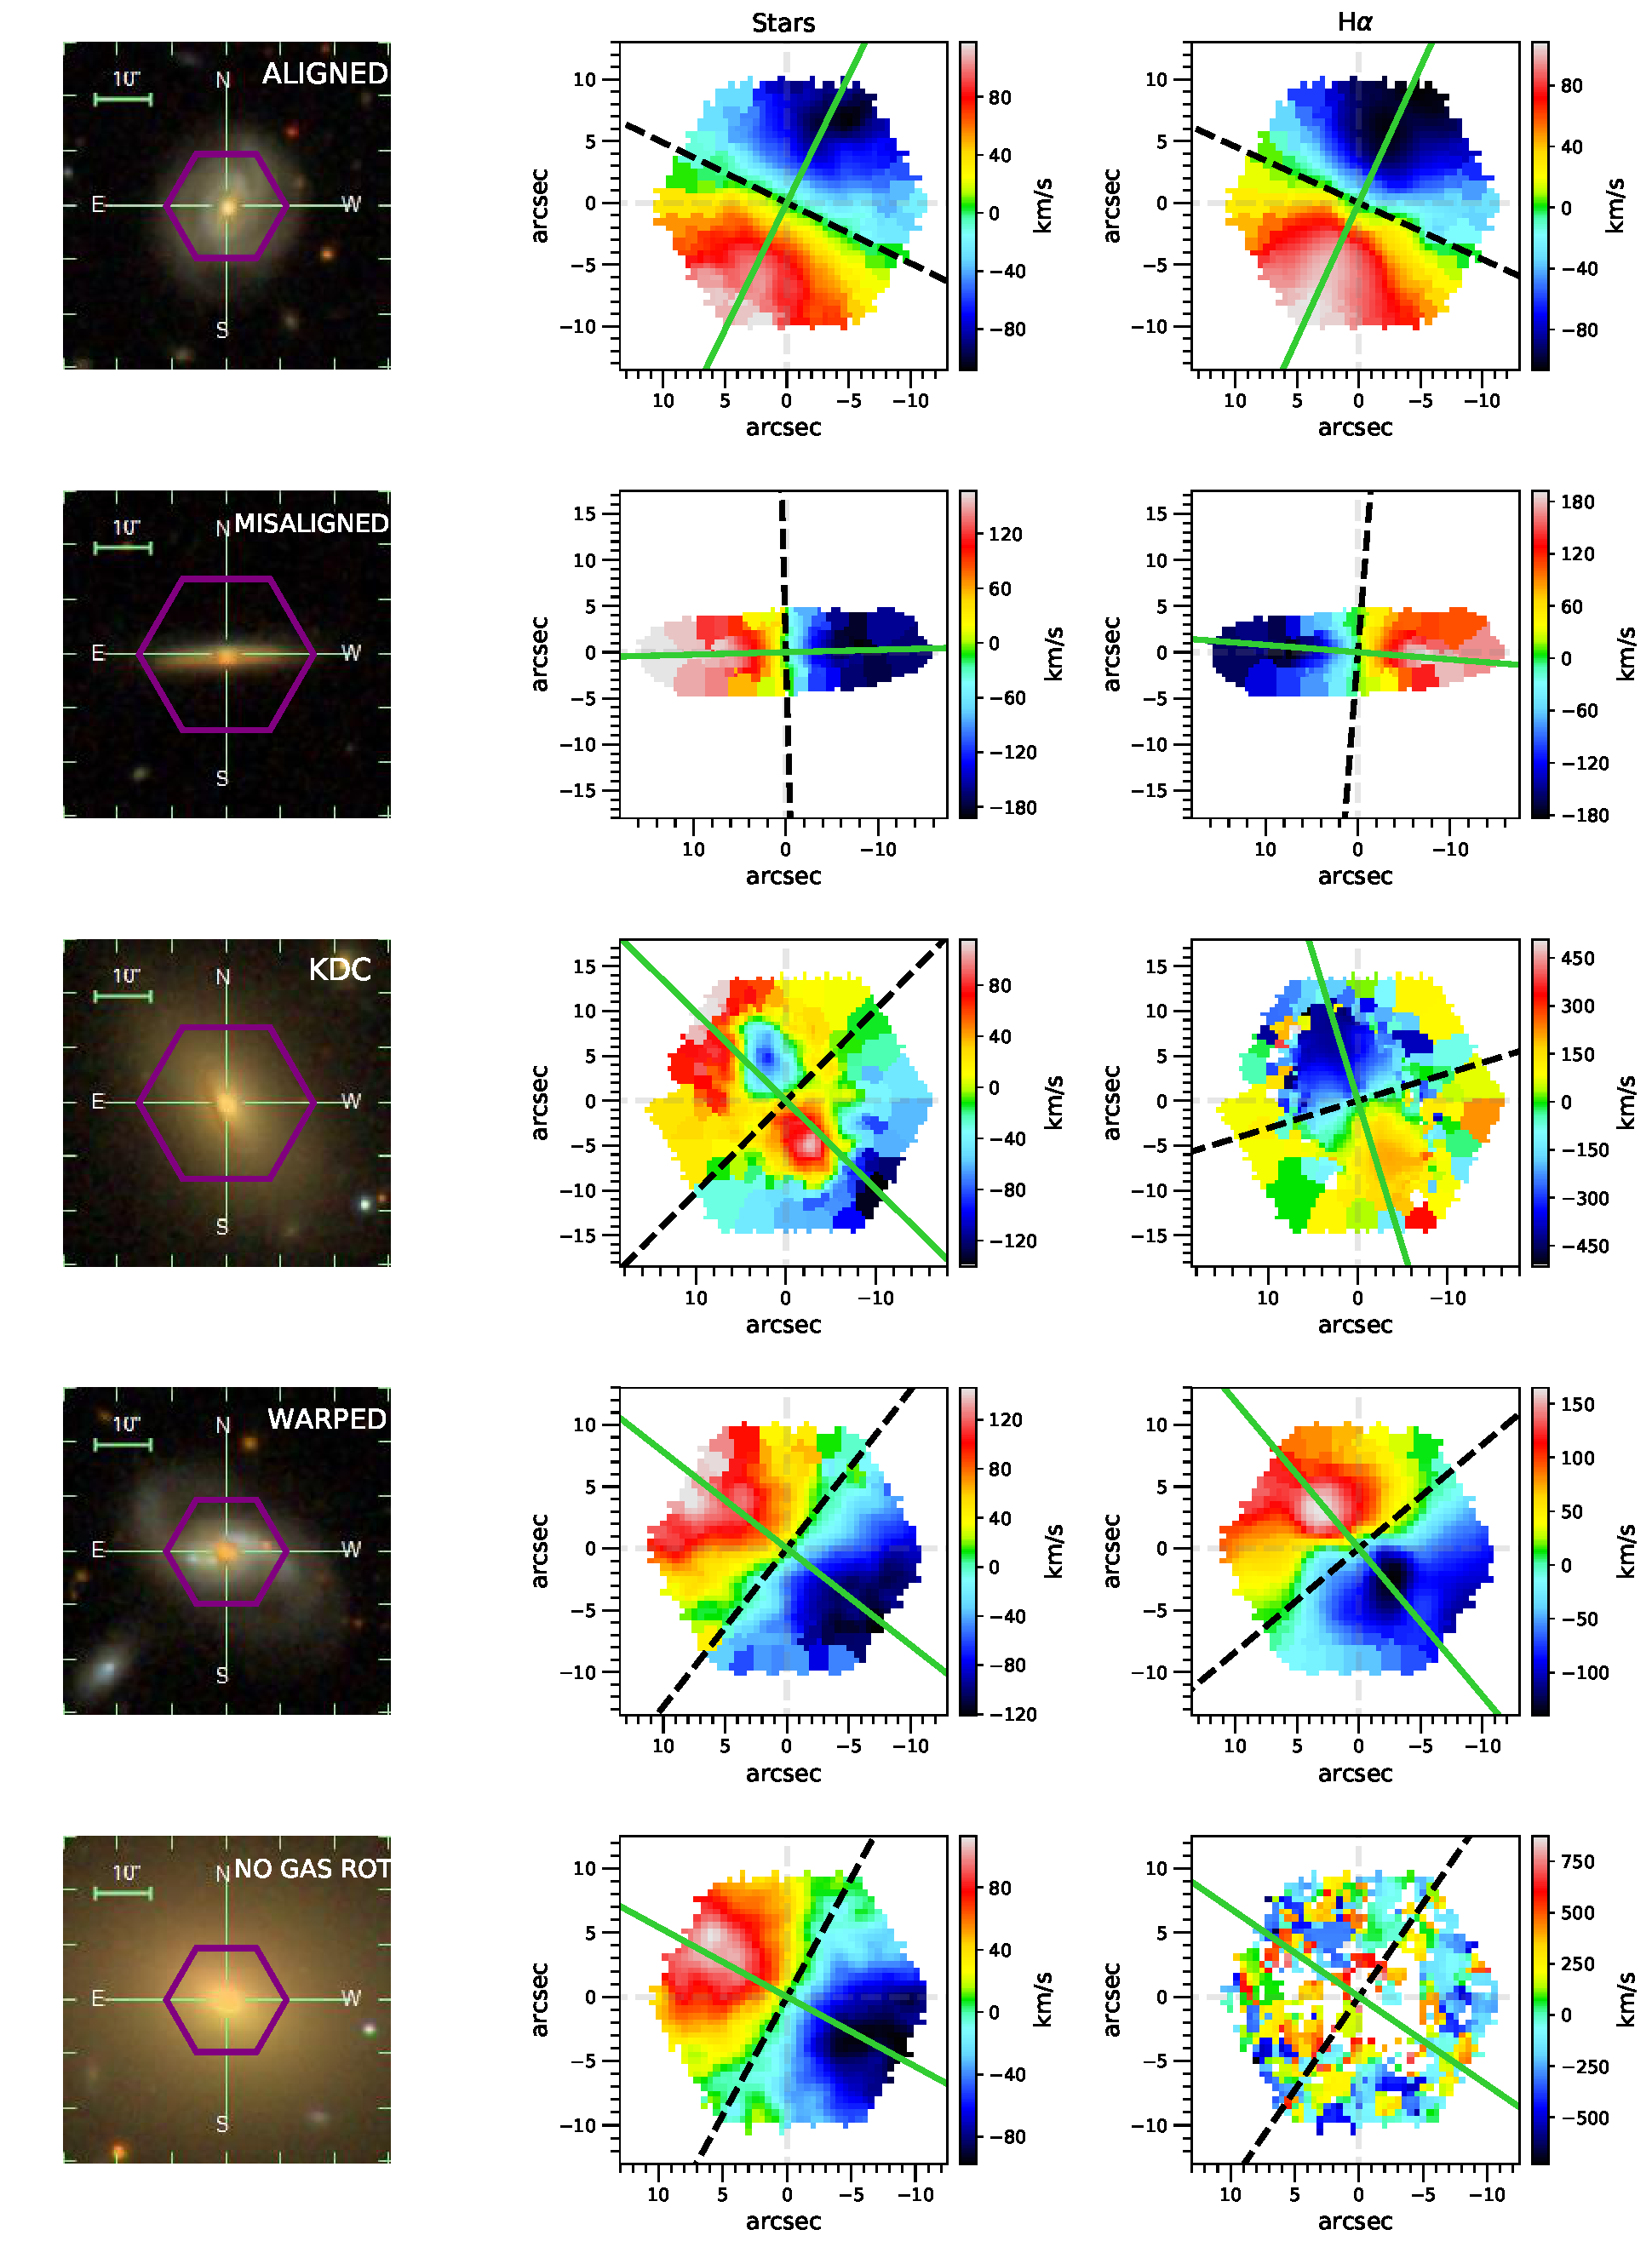
\includegraphics[width=0.8\linewidth]{misalignment_grid.pdf}
    \caption{Examples of PA fits for galaxies with different kinematic classifications. For each galaxy (row), we show the photometry taken from SDSS with the MaNGA IFU observation footprint overlaid in purple, the stellar velocity field and the H$\alpha$ velocity field. The kinematic PA fits (see \S\ref{sec:def_kin_mis}) are shown on the velocity fields (green solid line) with the axis of rotation (black dotted line). The kinematic classifications from top to bottom are; (a) PLATEIFU: 7958-6101, kinematically aligned near face on; (b) PLATEIFU: 8465-12704, counter-rotating near edge on; (c) PLATEIFU: 9868-12704, with a KDC in the stellar velocity; (d) PLATEIFU: 8252-6103, with a warped H$\alpha$ velocity field with respect to the stellar; (e) PLATEIFU: 10219-6102, with a centrally depleted/missing H$\alpha$ velocity field but coherent rotation in the stellar.}
    \label{fig:mis_grid}
\end{figure*}

\subsection{Defining kinematic misalignment} \label{sec:def_kin_mis}
Only selecting galaxies with dominant coherent rotation (both clean and messy) for both stellar and H$\alpha$ velocity fields with no defined features in either map, we are left with 3798 galaxies used in this analysis. The mass distribution of the $\Delta$PA defined sample with respect to MPL-8 is shown in Figure \ref{fig:samp_cons}. For the purpose of quantifying external interaction, we define the offset angle between the kinematic PAs of the stellar and ionized gas fields as such; 
\begin{equation} \label{eq:delPA}
\Delta PA = |PA_{stellar} - PA_{H\alpha}|. 
\end{equation}
We define galaxies with $\Delta$PA > 30$^{\circ}$ to be significantly kinematically misaligned. \green{why?}

\subsection{Morphology} \label{sec:morph_def}
We classify the morphology of $\Delta$PA defined MaNGA galaxies through the formalism laid out by the citizen science project; GalaxyZoo2 \citep[GZ2;][]{willett2013}. GZ2 provides visually identified morphologies (and also measures finer morphological features e.g. bars, bulge size and edge-on disks) for 304,122 galaxies drawn from SDSS. GZ2, however, is not complete for the MaNGA sample and has been combined with an unpublished version; GalaxyZoo4 with debiasing code re-run to provide a consistent set of definitions for all MaNGA targets (see; \url{https://www.sdss.org/dr15/data_access/value-added-catalogs/?vac_id=manga-morphologies-from-galaxy-zoo}). 

In a nutshell, GZ2 provides morphological classification through a decision tree of questions. Further questions are dependent on the answer to the previous to characterise a certain morphological type and identify finer features (see Figure 1 in \citep{willett2013} for this flowchart). From this, a table of vote fractions for each question combined with the total number of votes dictate a reliably sampled galaxy population with a set of desired morphological features. 

The first question in the decision tree 'Is the galaxy smooth and rounded with no sign of a disk?', allows categorisation into broad Early type (ETGs) and Late type galaxies (LTGs). We select galaxies with a debiased vote fraction > 0.7 for smooth to be ETGs and galaxies with a debiased vote fraction of > 0.7 for disk or features to be LTGs. \green{Should remove features?}. Defining an exact population of lenticular galaxies (S0s) is tricky through public classifications. LTGs, however, can be separated based on the dominance of the bulge with respect to the disk in GZ2 through the question 'How prominent is the central bulge, compared with the rest of the galaxy?'. \citep{willett2013} demonstrate a strong correlation between bulge dominance as defined per this question and expert classifications of T-type \citep{nair2010}. Equation 19 of \citet{willett2013} provides a linear mapping from GZ2 bulge classification to expert defined morphological T-type. Care must be taken in using this linear mapping \citep[see discussion in][]{willett2013}, however, this should be a reasonable parameterisation to coarsly separate LTGs into earlier-type (S0 - Sa) and later-type spirals (Sb - Sd). We split our LTG population at T-type = 3, to give three morphological categories along with pure ETGs. \green{Table with numbers of galaxies for each category.}

\subsection{Group membership and halo mass definitions}
To investigate different pathways leading to kinematic misalignment, we must separate galaxies into centrals and satellites and consider the size of the group that they reside in. 

We identify groups with an adaptive halo-based group finder of \citet{yang2005,yang2007} and with improved halo mass assigning techniques \citep[see;][for details and application to SDSS]{lim2017}. In a nutshell, the group finder uses either the stellar mass or luminosity of central galaxies in addition with the nth brightest/most massive satellite as proxies for halo mass. Galaxies are assigned to groups through an iterative process, where halo properties such as halo size and velocity dispersion are updated until membership converges. For groups that are outside of the redshift limit where groups are complete \green{$\sim 0.7$ for SDSS?}, final halo masses are assigned through abundance matching. Those incomplete are assigned halo masses based on the ranking between halo mass and the proxy found at the final iteration of the group finder.

The performance of the group finder has been tested on realistic mock catalogues, showing that the halo masses of individual haloes are consistent with the true mass with a typical scatter of $\sim$0.2 dex. This scatter is similar to the commonly used group finder of \citet{yang2007}, however extends uniformly to halo masses 0.7 dex lower. 

For this work, we use the stellar mass based halo mass proxy for the SDSS main sample. \citet{lim2017} do not apply the group finder to the thin strips in the Southern Galatic Cap of SDSS main due to incomplete groups resulting from close proximity to borders. MaNGA galaxies in these strips are therefore unclassified by the group finder, resulting in 5088 matched galaxies with halo mass estimates and group membership classifications into central or satellite.

\subsection{Pipe3D}
We use spatially resolved derived properties, such as SFR gradients, gas mass, $\lambda_{R}$... using the Pipe3D pipeline \citep{pipe3Da,pipe3Dvac}.

\subsection{IllustrisTNG}

\section{Results}
\subsection{Total population}
Firstly we consider all $\Delta$PA defined galaxies (i.e. selecting all stellar and H$\alpha$ velocity fields with clean or messy defined PAs) for MaNGA \red{and for our matched comparison sample in IllustrisTNG}. Figure \ref{fig:total_pa_dist}, shows the distribution of $\Delta$PA for MaNGA and IllustrisTNG. \red{Discussion about comparison between MaNGA and TNG}

\begin{figure}
	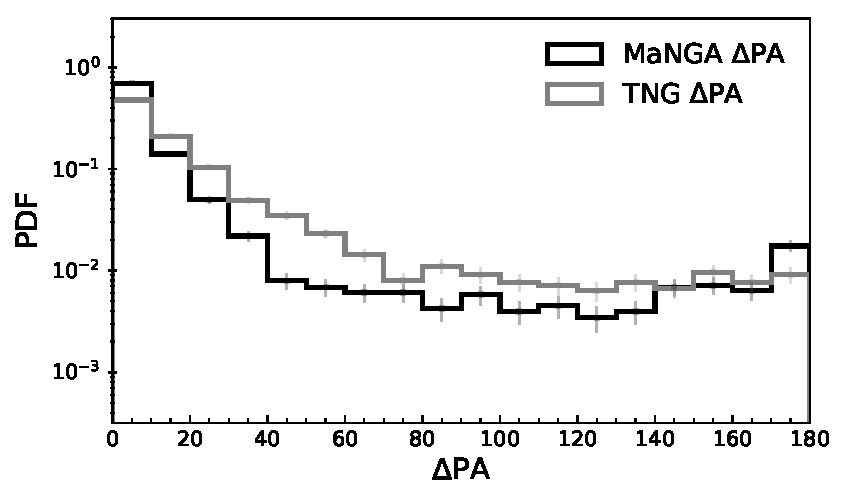
\includegraphics[width=\linewidth]{total_pop/mpl8_pa_dist.pdf}
    \caption{Probability density distribution of kinematic misalignment as defined by $\Delta$PA for the total MaNGA sample (black solid line) \red{and matched TNG-100 sample.} $\Delta$PA is strongly peaked around 0$^{\circ}$ with a small boost close to 180$^{\circ}$.}
    \label{fig:total_pa_dist}
\end{figure}

We now divide our MaNGA $\Delta$PA defined population at $\Delta$PA = 30$^{\circ}$ into aligned and misaligned (see \S\ref{sec:def_kin_mis} for choice of 30$^{\circ}$ reasoning). In the following, we also consider galaxies with defined stellar PAs but undefined H$\alpha$ due to central depletion or incoherent rotation/dispersion domination (NGRs). Figure \ref{fig:delPA_stelM} shows the distribution of stellar mass for these three populations. Kinematically aligned and misaligned galaxies appear to be consistent in stellar mass, whereas NGRs appear to be preferentially more massive. \citet{graham2018} previously demonstrated the tight correlation between stellar angular momentum and stellar mass for MaNGA (MPL-5; $\sim$2300 galaxies). Since NGRs are typically higher mass, it could be expected that they are less rotationally supported with respect to the $\Delta$PA defined populations. Figure \ref{fig:delPA_lambda_Re}, shows $\lambda_R$ vs $\epsilon$ for all $\Delta$PA defined galaxies and the medians for the aligned, misaligned and NGR samples. Kinematically aligned galaxies reside at preferentially higher $\lambda_R$ and ellipticity with respect to NGRs. This is indicative of the dispersion dominance over rotation for disrupted gas poor and typically higher mass galaxies that we see in our NGR sample. Interestingly, kinematically misaligned galaxies also typically reside close to the slow rotator regime (defined by the black solid line). This suggests that NGRs and kinematically misaligned galaxies have had similar levels of disruption to their angular momentum, most likely due to interactions and mergers, in their recent history. \red{NGRs more massive and hence would naturally expect them to reside closer to slow rotator regime in comparison to misaligned galaxies. Expand on this discussion.}

\begin{figure}
	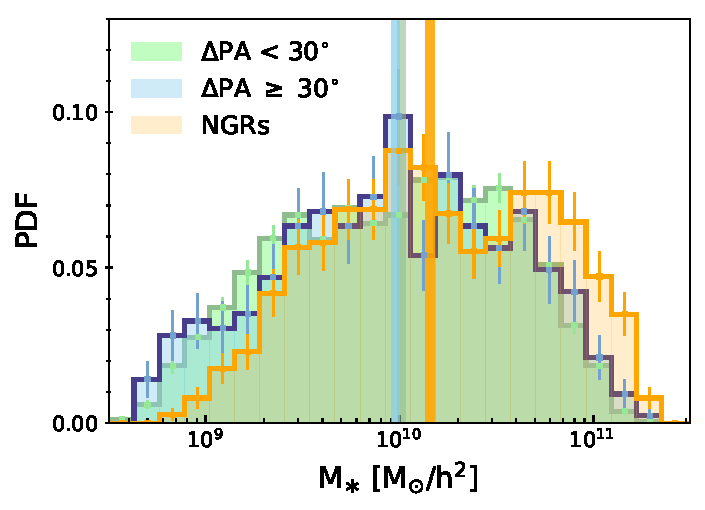
\includegraphics[width=\linewidth]{total_pop/delPA_stelM.pdf}
    \caption{Probability density distributions of stellar mass, $(M_{\ast}/M_{\odot})$ for aligned galaxies ($\Delta$PA < 30$^{\circ}$) shown with black (solid line), those with high misalignment ($\Delta$PA > 30$^{\circ}$) are in red (solid line) and NGRs are in green (dot-dashed line). Each histogram is given with Poisson errors on each bin. The vertical lines denote the corresponding distribution's median. Splitting on $\Delta$PA shows no marked difference in stellar mass, however, those without gas rotation are preferentially more massive.}
    \label{fig:delPA_stelM}
\end{figure}

\begin{figure*}
	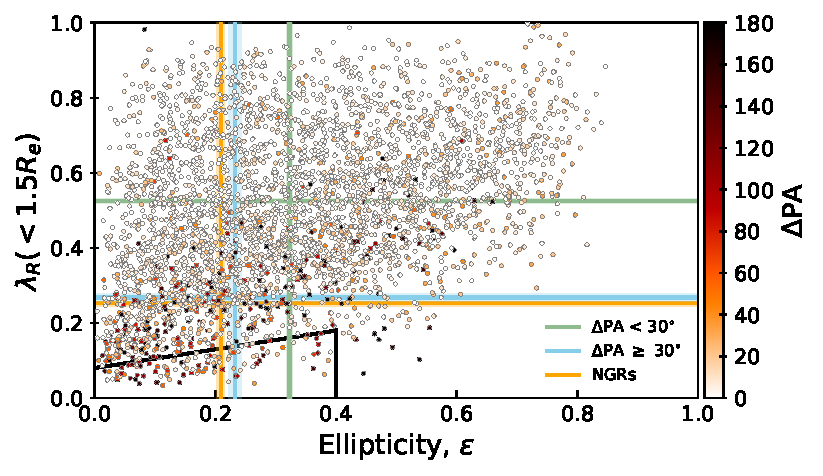
\includegraphics[width=\linewidth]{total_pop/delPA_lambda_Re.pdf}
    \caption{$\lambda_R$ within 1.5$R_e$ against ellipticity, $\epsilon$ for all galaxies with defined $\Delta$PA. Medians for kinematically aligned ($\Delta$PA < 30$^{\circ}$), misaligned ($\Delta$PA > 30$^{\circ}$) and NGR are shown by the black, red and green dashed lines respectively. Aligned galaxies reside more typically in the fast rotator regime with higher $\lambda_R$ and $\epsilon$, whereas misaligned galaxies and NGRs reside closer to the slow rotator regime.}
    \label{fig:delPA_lambda_Re}
\end{figure*}

\subsection{Morphology}
We now sub-divide the total population by morphology into ETGs, S0/Sas and Sb/Sds as defined in \S\ref{sec:morph_def}. Figure \ref{fig:morph_PA}, shows the distributions for each category. We find that for all morphological types, galaxies are most commonly aligned with strong peaks below $\Delta$PA $\sim 30^{\circ}$. ETGs show a flatter distribution than their later counterparts, as the most likely to exhibit misalignment. LTGs show deeper drop-offs above $\Delta$PA $\sim 40^{\circ}$, with a boost around $\Delta$PA = 180$^{\circ}$, seen most strongly for the Sb/Sds. We quantify the overall misalignment fractions in the first column of Table \ref{tab:mega_table}. This morphological difference in misalignment is likely a result of several factors. Gas rich LTGs have typically higher specific angular momentum, and hence, require a higher magnitude gas inflow to create an offset in rotation. Conversely, ETGs are more dispersion dominated and gas poor enabling smaller gas in-flows (or outflows) to create a kinematic misalignment. 

These misalignment fractions of ETGs are roughly consistent with previous findings in \red{ATLAS3D} and for LTGs similar to those found in \red{SAMI}. 

\red{The boost in the PDF around 180$^{\circ}$ suggests that near counter-rotation is a stable state for galaxies. This is seen most prominently in Sb/Sds. A possible explanation is that these rotation dominated galaxies host strong stellar torques, which act to realign gas on much faster timescales than in ETGs. Counter-rotators, however, remain stable and hence contribute proportionally higher to the misaligned distribution, as those at intermediate misalignments settle towards alignment. Stellar torques act to realign disrupted gas on the order of $\sim X$ dynamical timescales. Check $\lambda_{R}$ for counter-rots - are they lower ang mom due to significant disruption?!}

\begin{figure}
	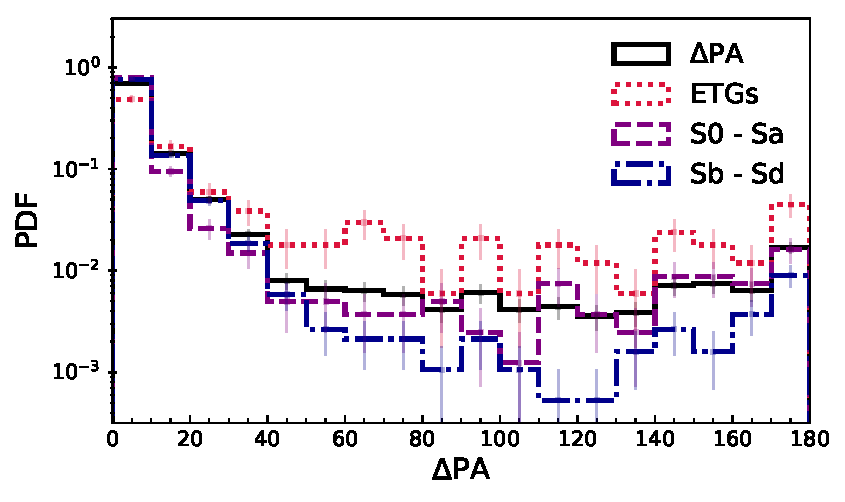
\includegraphics[width=\linewidth]{morph/delPA_morph.pdf}
    \caption{Probability density distributions of kinematic misalignment as defined by $\Delta$PA split on morphology. Distributions for the total population, ETGs, S0/Sa and Sb/Sds are shown by black solid, dotted red, dashed purple and dot-dashed blue lines respectively. Earlier type galaxies are more likely to be misaligned than later type galaxies. red{Add near counter-rotators to median lines.}}
    \label{fig:morph_PA}
\end{figure}

\begin{figure}
	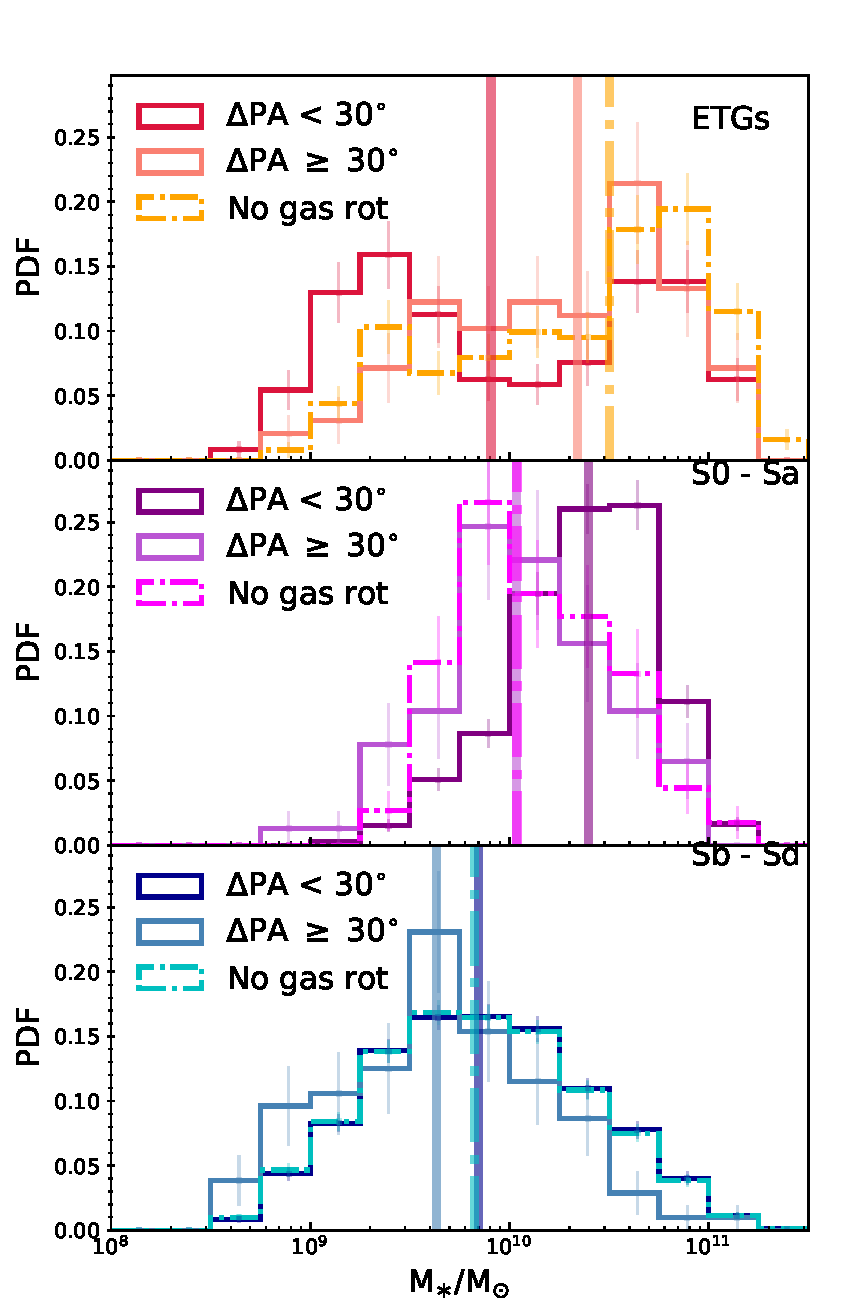
\includegraphics[width=\linewidth]{morph/delPA_stelM_morph.pdf}
    \caption{Probability density distributions of stellar mass, $(M_{\ast}/M_{\odot})$ for aligned galaxies ($\Delta$PA < 30$^{\circ}$, misaligned galaxies ($\Delta$PA > 30$^{\circ}$) and NGRs for ETGs, S0/Sas and Sb/Sds (top to bottom). In each panel the aligned/misaligned are shown with solid lines with the aligned in the darker shade. NGRS are shown by dot-dashed lines. Each histogram is given with Poisson errors on each bin. The vertical lines denote the corresponding distribution's median. For ETGs, aligned galaxies are less massive than the misaligned sample. This trend, however, reverses for S0/Sas and Sb/Sds.}
    \label{fig:morph_stelM}
\end{figure}

\subsection{Group membership}

\begin{figure*}
	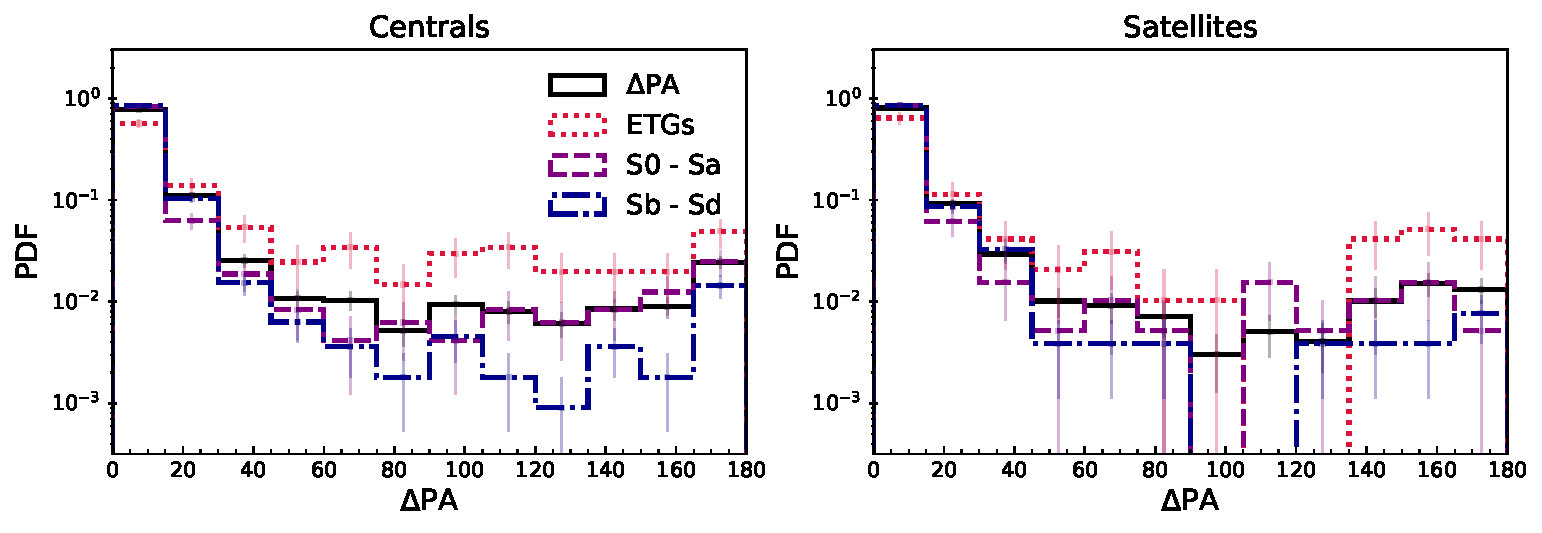
\includegraphics[width=\linewidth]{cen_sat/delPA_morph_lim.pdf}
    \caption{Same as Figure \ref{fig:morph_PA}, however split by group membership into centrals (left) and satellites (right).}
    \label{fig:group_morph_PA}
\end{figure*}

\begin{figure*}
	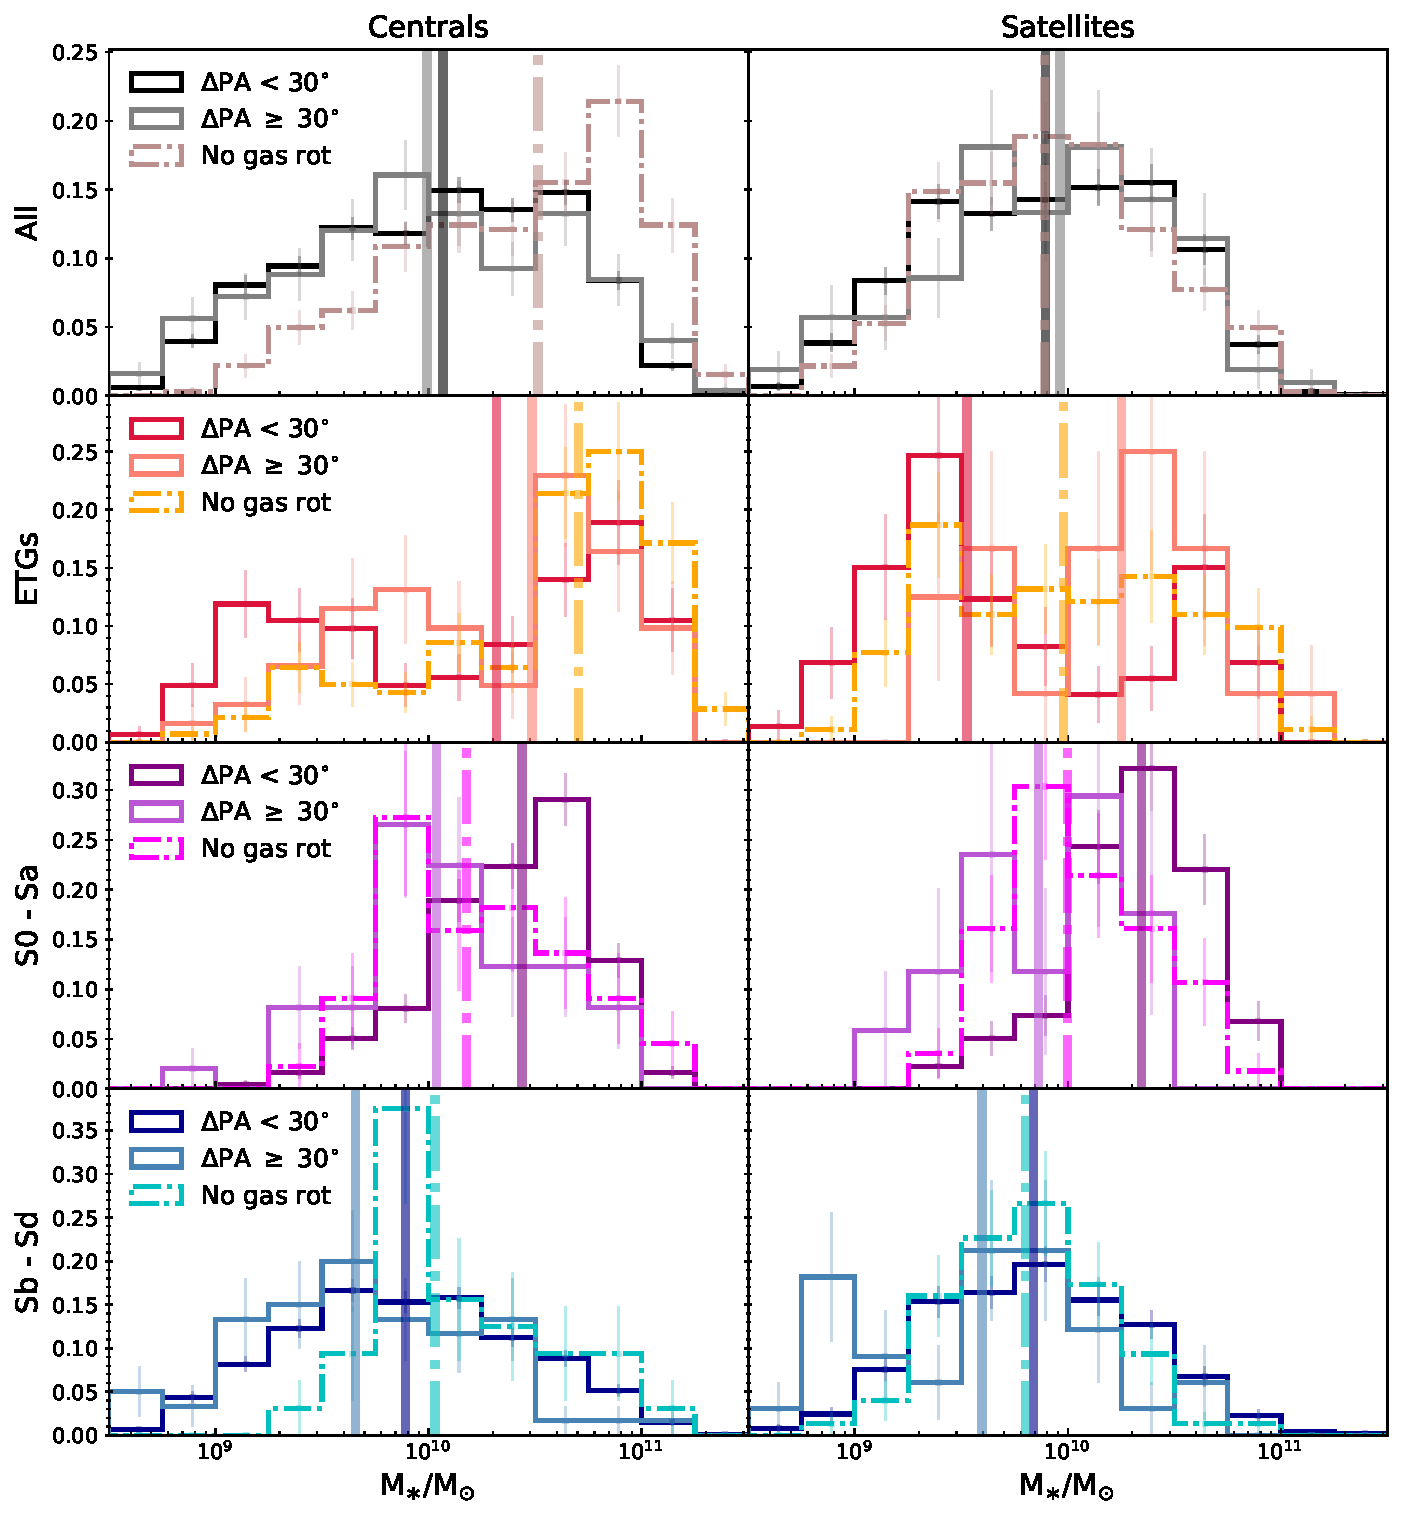
\includegraphics[width=\linewidth]{cen_sat/delPA_stelM_morph_lim.pdf}
    \caption{Same as Figure \ref{fig:morph_stelM}, however split by group membership into centrals (left) and satellites (right). \red{We see that...}}
    \label{fig:group_morph_stelM}
\end{figure*}

\begin{table}
\begin{tabular}{llll}
\hline
          &           All &      Centrals &    Satellites \\
\hline
      All &  11.1\% (3798) &  11.5\% (2185) &  10.1\% (1007) \\
     ETGs &   27.9\% (301) &   29.4\% (204) &    24.7\% (97) \\
 S0 - Sas &    9.7\% (677) &   10.1\% (483) &    8.8\% (194) \\
 Sb - Sds &   5.4\% (1634) &   5.2\% (1112) &    5.7\% (522) \\
\end{tabular}
\caption{}
\label{tab:mega_table}
\end{table}

\bibliographystyle{mnras}
\bibliography{biblio.bib}

%%%%%%%%%%%%%%%%%%%%%%%%%%%%%%%%%%%%%%%%%%%%%%%%%%

%%%%%%%%%%%%%%%%% APPENDICES %%%%%%%%%%%%%%%%%%%%%
\section*{Acknowledgements}
This project makes use of the MaNGA-Pipe3D dataproducts. We thank the IA-UNAM MaNGA team for creating this catalogue, and the ConaCyt-180125 project for supporting them

\appendix

\section{Some extra material}

If you want to present additional material which would interrupt the flow of the main paper,
it can be placed in an Appendix which appears after the list of references.

%%%%%%%%%%%%%%%%%%%%%%%%%%%%%%%%%%%%%%%%%%%%%%%%%%


% Don't change these lines
\bsp	% typesetting comment
\label{lastpage}
\end{document}

% End of mnras_template.tex